\chapter{Background}\label{ch:background}

In the first section, we are going to introduce some basics of the design in seL4, then move on to the next section where defines the challenge that we are going to solve in this thesis. In the final section, we will introduce some related projects that provide emulation at ISA, ABI, and API layers,and then discuss their trade-offs. We will first introduce an existing solution to the problem that we face using QEMU. Then we will introduce other three related projects from the API layer emulation approach using Cygwin down to ABI layer emulation approaches provided by Wine and UML.      

\vspace*{-\dimexpr1.0ex+0.1\baselineskip\relax}

\section{Overview of seL4}

seL4 has been formally verified for correctness (\cite{Klein_EHACDEEKNSTW_09}) and is the fastest microkernel in the world. seL4 adheres to the principle of $minimality$, only provides the critical kernel functionalities that can't be achieved in the user-level implementation. Such design minimizes the TCB in seL4, making it possible to be formally verified. seL4 was born for safety. The componentized system architecture that seL4 implements enforce the isolation between those untrusted components and other trusted components running on top of the kernel. With the fine-grained capability-based access control model seL4 can carefully manage the access to the hardware resources from the software components. In this section, we will present the current state of relevant seL4 features to motivate this thesis. First, we will introduce the powerful and robust capability system in seL4. Then we will introduce the system calls in seL4 and the resource management. Finally, we will introduce the scheduling system in seL4.

% (Fixed: Formal descriptio of seL4!)

\subsection{Cpabilities}

In seL4, the access rights to any resources are represented by capabilities. When the kernel launches the initial task, which is the $root task$, the capabilities to all the resources are also handed to it. The root task is the first seL4 user-level thread which will take care of the resource allocation in the future. Capabilities reside in the seL4 capability space also called $cspace$, which consists of several capability nodes called $cnodes$, each $cnode$ is a table that has several slots. Those slots can contain either capability to the next $cnode$ or a capability to a kernel resource or be empty. Hence, $cnodes$ form a directed graph in the $cspace$. The $cspace$ maps the access rights to kernel object identifiers. Resolving the capability requires resolving the $cspace$ address to find the final slot. According to the seL4 semantics, there are several operations to manipulate capabilities for different purposes, such as copy, mint with a badge, move, mutate with a badge, delete or revoke, etc. When the capability is copied or minted with a specific unforgeable token called a badge, it's said to be derived. However, not all the capabilities can be derived. The seL4 kernel will keep track of the capability derivation via the capability derivation tree to delete a capability (only remove such capability from the $cnode$) or revoke (also remove all the capabilities derived from such capability) it later.

\subsection{Communication}

The seL4 provides both synchronous and asynchronous communication methods through IPC via endpoints and notifications via notification objects. 

\subsubsection{IPC}

In the seL4, two threads can communicate with each other via either a blocking fashion or a non-blocking fashion over an endpoint. It can be a one-way message passing from sender to the receiver, or a two-way fashion which implements a $rendezvous$ model, where the sender will wait for a reply from the receiver. In the design of seL4, to send the message via IPC, the sender must specify the length of the message payload. If the message payload is large, then it will be stored in each thread's IPC buffer, and the kernel will copy the payload from the sender's buffer to the receiver's buffer, while if it is small, no memory copy is required, the message payload will be stored in the registers instead to improve performance. In seL4 the system calls are mainly for communication, they are $seL4_Send$, $seL4_NBSend$, $seL4_Call$, $seL4_Reply$, $seL4_Recv$, $seL4_NBRecv$, and $seL4_Yield$. The first four are sending system calls, the middle two are receiving system calls and the last one is the schduling system call. Most of other methods for manipulating the kernel objects are implemented using those critical system calls. Since the IPC mechanisms are critical to the performance in seL4, seL4 implements a fast code path to further optimize the IPC performnace when several conditions are satisfied. In general, those conditions are: 

\begin{enumerate}
    \item the sender is using $seL4_Call$ or the receiver is using $seL4_ReplyRecv$,
    \item No capbilities should be transferred,
    \item The data in the message must fit into the $seL4_FastMessageRegisters$ registers without using IPC buffer,
    \item the receiver has a valid address space without any memory faults,
    \item the receiver has the highest priority among all the threads in the scheduler,
\end{enumerate}

Besides the system calls, the seL4 also utilities IPC between teh kernel and the receiver to handle the thread faults. In the seL4, when a thread generates a thread fault, the kernel will suspend the execution of the faulting thread and constructs a message, which contains the information about the faulting thread, then send the message to the specific endpoint where a fault handler thread is waiting on. After the fault handler corrects the anomaly, it can either explicitly tell the kernel to resume the faulting thread or invoke the reply object to inform the kernel. 

\subsubsection{Notification}

The notification mechanism provides an asynchronous method for seL4 threads to send signals to each other. It is primarily used for handling the interrupt and maintain synchronisation between threads. The notification object can have three states: waiting, active or idle, and it consists of a word of data, where the badge will be stored and accumulated if no threads are waiting on it. By using notification objects, a thread can poll or block on an interrupt. On the other hand, a notification object can also be bound to the thread so that the thread can receive the notification issued while blocking on the endpoint waiting for IPC. Such design avoids using one dedicated thread for receiving IPCs and the other one for receiving notifications.

\subsection{Memory Management}

Since the design seL4 adheres to the $minimality principle$, the seL4 kernel itself doesn't handle the memory management. Such OS services are implemented at the user level. When the kernel boots, it will first allocate a small, static amount of memory for itself. Those memories have already been mapped so that the kernel can directly access them. However, the size of such memory is platform-specific. Then it will start the $root task$, and pass the untyped physical memory along with the capabilities to all the resources to the root task. Those untyped memories can be retyped into different kernel objects such as $cnodes$, $frames$, $page tables$, etc. With such a design, it's very flexible for the system developer to decide the specific memory layout. However, no fixed-size data structure can be used in the kernel as the kernel can't assume the memory layout.

\subsection{Scheduling}

In the seL4's implementation, the kernel will choose the head of the list queued at the scheduler with the highest priority as the next thread to run. To lookup for the highest priority efficiently, seL4 uses a two-level bit field to track the priority lists consisting of runnable threads in the schedular. The first level of the bit field divides the priority levels into several sets, each bit represents a set of the priority levels. Also, it is the index to the second-level bit field array. Each bit in the entry of the second-level bit filed array maps a priority level in the current set. Such data structure ensures only two words need to be resolved to get the highest priority.

\subsubsection{Traditional Scheduling}

In seL4, there are two main scheduling policies, the first policy is the traditional one that implements a round-robin scheduler with 256 priority levels. Each thread has two attributes, a maximum controlled priority and an effective priority which must be less than the maximum controlled priority. The priority levels can be changed through the thread's capabilities. A Thread can run until it exhausts its timeslice or gets preempted by the other threads with higher priorities, or it can give up the execution manually by calling $seL4_yield$.

\subsubsection{MCS scheduling}

In the traditional seL4, the schedular prioritizes the thread with the highest priority, which means if the thread happens to be the only one with the highest priority, it will monopolise the CPU unless a thread with higher priority occurs or it finishes its task. To overcome such a problem, seL4 introduces its own MCS scheduling. The seL4's MCS scheduling can be enabled by changing the configuration when building the kernel. In the implementation of the seL4's MCS, each thread has a scheduling context that contains a budget that determines how long the thread can run and a period that determines how often the thread can run. (TODO: MCS paper). Those two attributes form an upper bound of the thread's execution time and prevent the high-priority thread from monopolising the CPU. The seL4's MCS scheduling mechanism allows it to provide strong time resources isolation to the components with different criticalities besides the space resources isolated which are guaranteed by capabilities. Therefore, seL4 offers great support for real-time systems.

\section{Challenge}

The secure and well design of the seL4 microkernel together with the formal verification ensure the kernel itself is robust and is the ideal foundation to build a secure system on top of it (\cite{Klein_AEHCDEEKNSTW_10}). What's more, seL4 is not only secure but also fast. With its performant IPC mechanisms and most advanced mixed critical real-time systems (\cite{Lyons_Heiser_14}) (TODO: use the new paper), seL4 is capable of handling a wide range of real-world scenarios. However, seL4 is relatively young compared to other mainstream kernels such as Linux, and its ecosystem is still growing. For those seL4 developers, there are limited tools that can be used to develop seL4-based systems or applications. On the other hand, Linux provides us a powerful development environment with many useful tools. Therefore, the main motivation of this project is to explore some ways to leverage the Linux development tools to make developing seL4 systems much easier and faster.

But developing applications targeted for seL4 in Linux is challenging because seL4 as a microkernel has different semantics and OS model compared to Linux (in figure \ref{fig:osmodel}).

\begin{figure}[h] % (Fixed: fix the bad scaling problem)
    \centering
    \copyrightbox[b]{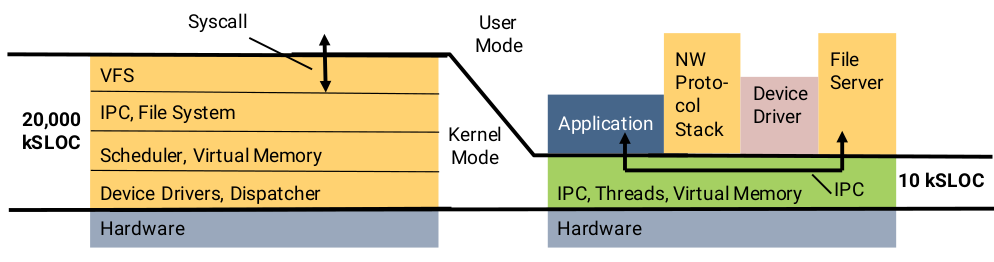
\includegraphics[scale=0.4]{ch2/OS models.png}} % 
    {Source: "The seL4 Microkernel – An Introduction" (p. 3), by Gernot Heiser, 2020, the seL4 foundation. Copyright  under the Creative Commons Attribution-ShareAlike 4.0 International (CC BY-SA 4.0) License.}
    
    \caption{Linux based OS model vs seL4 based OS model.}
    % {\tiny Note: The picture comparison between monolithic OS vs microkernel OS model. Reprinted from "The seL4 Microkernel – An Introduction" (p. 3), by Gernot Heiser, 2020, the seL4 foundation. Copyright  under the Creative Commons Attribution-ShareAlike 4.0 International (CC BY-SA 4.0) License.}
    \label{fig:osmodel}
\end{figure}

Linux is a monolithic kernel that provides a wide range of OS services. The drivers and many OS components are implemented inside of the kernel. Many those OS services execute in kernel mode. In contrast, seL4 is just a thin wrapper of the CPU, providing minimal critical services of the hardware resources, and thus it guarantees strong isolation of different OS components. The OS services are implemented at the user level as separate components. Such design minimizes the TCB. 

In a monolithic kernel, the user-level applications request the OS services through the system call interfaces. A system call will cause a context switch from the user mode to the kernel mode, and the kernel will serve the OS requests by itself. For example, an I/O request from the user level will trigger the system call and the kernel will dispatch such request to the corresponding handler. In Linux, this might be a handler in the VFS layer. Then the VFS layer handler will find the particular file system handler to perform the I/O. However, in the seL4 based OS model, it works differently. First, to clarify the term, we are going to call anything that runs in seL4 user level as "seL4 applications". Also, we will classify those applications that request OS services as "client applications" and those applications that provide OS services as "server applications". When the seL4 client applications request OS services, it will invoke IPC mechanisms provided by the seL4 kernel. The seL4 IPC is a synchronous or asynchronous method for transmitting small amounts of data and capabilities between seL4 threads. seL4 applications can invoke seL4 IPC mechanism by calling a seL4 system call, which triggers the context switch to the kernel mode, and the seL4 microkernel will then transport the input to the designated seL4 server application via the endpoint. Those requests are served by the seL4 server application at the user level. The seL4 client applications and seL4 server applications are isolated components, which ensures the security of the whole system.

As we can see, the main problem here is that seL4 and Linux have different semantics and program flow of serving OS services, the final goal of this project will be providing methods for developing seL4 user-level applications which can either run on Linux or seL4. In other words, we need to provide compatibility between seL4 applications and Linux.

\section{Related Work}

% (Fixed: I would expect this to lead off with a discussion on the various abstraction levels we have, and that emulation can happen at each of them)

In this section, we are going to introduce several related projects which provide emulation at different levels from ISA layer to API layer. First, we will present an existing solution to the challenge we stated before, which uses QEMU to provide an full system emulation. Then we will present an API-level emulation project called Cygwin and two ABI-level emulation approaches called Wine and UML. 

\subsection{Full system emulation}

The full system emulation provides a way to run an unmodified target binary code, such as applications or even operating systems like Linux or Windows on a host machine, even if the emulated target is compiled for different ISA from the host's.

\subsubsection{QEMU}

% (Fixed: This whole section is highly confusing, mangling hardware virtualisation with dynamic translation. This needs much better explanation and classification that these are two completely separate operating modes
Also, the"more efficient" claim is unsubstantiated
Really, this is virtualising at the ISA level, and is just one approach to that)

QEMU is a full system emulator supporting a wide range of ISA, and QEMU can also act as a virtualisation hypervisor if the guest's ISA is the same as host's ISA and the host supports Linux KVM (\cite{enwikiqemu}). By using a full system emulator such as QEMU, we can readily run the seL4 microkernel and its applications on top of Linux, and from the seL4 user-level applications' view, they are still running on top of the seL4 microkernel. 

(TODO: new QEMU uses TCG doesn't use GCC at all)
QEMU is a machine emulator, which means it can use portable dynamic translation to emulate an entire machine, including its processors and peripherals. To convert the guest instruction set into the host instruction set, QEMU will perform two phases. The first phase is the translation and the second phase is the code generation. In the first phase, QEMU splits each target CPU instruction into a few instructions called micro-operations. Each micro-operation is implemented using a small piece of C code that will be compiled by GCC to an object file later. A novel design in QEMU is that QEMU uses dummy code relocations generated by GCC as a place holder with a prefix \emph{$\_\_op\_param$} in the micro-operations, and patches it later when the code generator runs. Because some constants parameters in the target instructions are only known in the runtime. Those relocations can also be references to static data or functions. After that, the \emph{dyngen} will be invoked to generate the dynamic code generator. It will parse the previously generated object file depends on the host operating system's object file format, such as ELF in Linux, to get the symbol table, relocations, and code sections and use that information as the input to generate a dynamic code generator. In the second phase, the dynamic code generator will copy the stream of micro-operations into the host code section and patch the relocations with the runtime parameters. Those relocation patches are host-specific. For optimization, QEMU will maintain a fixed size cache to hold the recently translated blocks of instructions. 

Since QEMU can emulate CPU using dynamic binary translation, this means that QEMU have great flexibility, such as allowing binary code, such as running ARM binary on x86. However, emulation using dynamic binary translation introduces a massive performance overhead, therefore, recent versions of QEMU can leverage hardware virtualisation, such as Intel VT-x or AMD-V, which are supported by modern processors to to allow full system virtualisation at near native speed. These technologies may directly map a slice of the physical CPU to the virtual CPU (TODO: when to map?). Hence, the instructions of the virtual CPU can directly execute on the physical CPU slice. In Linux, QEMU leverages KVM to access CPU virtualisation extensions. However, since KVM is a driver for the physical CPU capabilities, this approach is very tightly associated with the CPU architecture and/or ISA. It means that the benefits of hardware acceleration will be available only if the target system is targetting the same ISA as the host's and the host processor supports hardware virtualization feature. Moreover, though QEMU provides its debugging interfaces to debug the guest system in a single stepping mode.

Although QEMU is an existing solution to emulate the seL4 system in Linux at the ISA layer, it's not an optimal option for emulating a high-performance microkernel like seL4 because of the overhead of hardware virtualization or machine emulation. In the former case, if the guest system such as our seL4 performs a privileged instruction, then it will trigger a trigger a world switch to the host (e.g. VMEXIT) to the host, and such overhead is not negligible. In the latter case, if QEMU resorts to dynamic binary translation, then it will have to perform a full machine emulation and translate the ISA into the host's ISA, which introduces significant overhead. However, the design goal of QEMU focuses on low-level machine emulation. It's helpful to inspect each instruction's execution of the CPU, but it's hard to use from a high-level seL4 developers' perspective. Because the debugger is not OS aware, the guest OS's context switch might confuse the debugger and lead to a breakpoint missing or a wrong variable value issue. In the following sections, we will introduce other approaches performing emulation at different layers, and then propose approaches used in this thesis to tackle the problem that we stated before in chapter \ref{ch:approaches}.


\subsection{API-level Emulation}

As we mentioned before, the ISA-level emulation involves emulating the emtire machine or using virtualization technologies, which introduces non-negligible overhead. In this section, we will introduce a project which performs emulation approach at the API layer to provide compatibility between two different systems.

\subsubsection{Cygwin}

% Cygwin32: A Free Win32 Porting Layer for Unix Applications

Cygwin is a compatibility layer that allows Unix-like applications to run on top of Windows (\cite{enwikicygwin}). This is achieved by introducing a DLL called cygwin1.dll which acts as an emulation layer providing substantial POSIX system call functionalities providing a Unix semantics. Cygwin also provides several standard Unix utilities such as bash, etc.

(TODO: diagram of the architecture)
Cygwin began development in 1995 at Cygnus Solutions. In the project, developers provided interfaces called Cygwin API to add the missing Unix-like functionalities in Win32 API, such as fork, signals, select, etc (\cite{Cygwin}). Cygwin will not magically make any POSIX application's binary code runnable on top  Windows directly. Executing those POSIX applications require the recompilation of the application. source code of the POSIX application can be recompiled using Cygwin and linked with DLL which implements the POSIX system call semantics using the Win32 APIs and native NT APIs. After executing the application, the Cygwin DLL will be loaded into the application's test region so that it has full access to the whole process. Next, shared memory is created containing the instances of the resources that the shared library can access. Therefore, the OS resources such as file descriptors can be tracked. Besides such shared memory regions, each process also has its resource bookkeeping structures, such as signal masks, PID, etc.

Cygwin has several nice designs to implement the POSIX features in Windows. For example, it handles signals by starting a separate thread from the library for only signal handling purposes. This thread waits for the Windows event used to pass signals to the process, and scan through its signal bitmask to handle the signals appropriately. However such thread resides in the same address space as the executing program, the signal sending function for sending a signal to other processes is wrapped with a mutex, and the signal sending function which sends the signal to itself is wrapped by separate semaphore or event pair to avoid them being interrupted. 

Another example is the implementation of sockets. They are mapped on top of the Winsock. However, Unix domain socket is not provided in Windows, so Cygwin implements it with the local IPv4 as the address family. Besides, Cygwin provides the Winsock initialization on the fly, as the Winsock requires to be initialized before the socket function is called. For implementing the POSIX $select$, Cygwin implements the polling of file handles besides socket type handles by sorting the file descriptors into different types and creating a thread for each type of the file descriptors present to poll those file descriptors with Win32 API. Such a design is because the Winsock only works on socket type file descriptors.

% (Fixed: mention somtimes the implementation of the emulation can be complex because of the poor mapping between two systems.)              

The API layer emulation requires to utilize the host systems' functionalities, but it's difficult to find an appropriate functions provided by the host systems sometimes. For example, in Unix-like systems, the $fork()$ system call provides a way to create a child process that copies the parent's address space, but there are no appropriate process creation functions in Windows which can be mapped on top of it, so the implementation of $fork()$ in Cygwin is relatively complex.  

Implementing $fork()$ semantics in Windows requiring to copy all of the executable binary and all the DLLs loaded statically or dynamically to be identical as to when the parent process has started or loaded a DLL. This can be problematic as Windows allows the binaries to be renamed to even removed to the recycle bin while the binary is executing, which means they can reside in a different directory or have a different file name. However, an executing process has to access to the binary files via the original filenames to fork its child processes. The solution to this problem is that Cygwin will try to create a private directory that contains the hardlink to the original files and remove it when no process is using it. When the parent process wants to fork a child process, it will first initialize a space in Cygwin process table for the child and create a suspended child process using Win32 CreateProcess API. 

After that, the parent process will use setjump to save the context and set a pointer to the current context in the Cygwin shared memory, and fill the child process's .data and .bss section with its own address space. Next, the parent process will block on a mutex and the child process will run and use the longjump to jump to the saved jump buffer. Then child process will release the mutex that the parent is blocked on and waits for another mutex. The parent process will copy its stack and heap into the child process space then release the mutex that the child is blocking on and return from the fork call. Finally, the child process will wake up and recreates any memory-mapped areas that passed to it and return from the fork call. However, such implementation is not perfectly reliable as in Windows, Windows implements the ASLR starting from Vista, which means the stack, heap, text, and other regions may be placed in different places in each process. This behavior interferes with the POSIX fork's semantic that is the child process has the same address space as the parent process. In that case, Cygwin will try to compensate the movable memory regions at the wrong place but can't do anything with those unmovable regions such as the memory heap.

In summary, adding compatibility at the API layer can solve most of the problems when attempting to run applications from foreign systems. While the downside is that, apparently this will only work when the user of Cygwin can obtain the source code of the application. Meanwhile, it's very difficult to implement every POSIX system call in Windows correctly due to the huge difference in the internal design between the two systems. 

Even though Cygwin can be used to run POSIX applications on Windows NT environment, we can still leverage the nice idea that Cygwin uses. To emulate seL4 in Linux we can link applications to a specific library that remaps the libseL4 APIs with the underlying host's system calls.

\subsection{ABI-level Emulation}

In the previous section, we have introduced Cygwin, which is an API-compatible solution for providing compatibility between Windows and Linux. However, the downside is that it's not binary compatible as we have to obtain the POSIX application's source code first and recompile it. In that case,  if we can't obtain the source code or the application that we want to emulate directly invokes system calls instead of calling them via the standard libraries, then it's impossible to perform the emulation. Hence, in this section, we will introduce two ABI-level emulations which are binary compatible.

\subsubsection{Wine}

% https://en.wikipedia.org/wiki/Wine_(software)#Basic_architecture
% (Fixed: Need to be improved, add more internals related to Wine)

(TODO: 

1. Win and Linux has different ABI, ELF and SysV ABI conventions, Win uses PE with its own ABI system, fastcall, cdecl, etc. 

2. Wine -> compatibility layer entirely in the user mode. Custom peloader.

3. Majority of the Win app doesn't use system call directly,  but instead calls "personality layer" <- the most popular one is Win32. 

4. Explain again how seL4 apps are typically coded this way by using libseL4-API. 

5. Wine provides API compatibility DLLs so that the Win32 apps will be linked to these DLLs instead and thus calling Wine's internal function, which translates such calls to POSIX equivalent or so. 

First example that provides the compatibility layer to run Windows applications in Unix-like operating systems is called Wine (\cite{enwikiWine}). However, Wine doesn't emulate the internal Windows logic like a virtual machine or an emulator. Instead, it directly translates the Windows ABI into POSIX-compliant calls. Besides, Wine also provides various Windows services through Wineserver as well as other Windows components. In Wine's architecture, it implements Windows's ABI entirely in the user space, rather than a kernel module. 

A system call from a Windows application usually invokes a particular DLL library, which in turn invokes the user-mode GDI/user32 libraries, and then finally invokes the system calls via Win32 subsystem. However, since the architecture of Windows OS is a hybrid model of monolithic kernel combined with the microkernel, some OS services run as separate processes, so applications need to invoke RPCs to communicate the user-mode services. In that case, this is somehow similar to how seL4 applications request OS services. Although Wine implements the Wineserver to provide services that are provided by the Windows kernel, as well as other OS functionalities, it's impossible to implement all the aspects of the Windows kernel as well as to use native Windows drivers due to the internal architecture of Wine. 

In Wine's architecture, the critical libraries are implemented using shared libraries and loaded dynamically at runtime, while in the seL4 system, all the binary codes are statically linked. So we can't imitate Wine's architecture and implementation. However, with a similar idea as the Wine project, we can still target the emulation layer of seL4 applications at the kernel ABI layer to achieve binary compatibility.

\subsubsection{User-mode Linux}

% (Fixed: This whole section suffers from being written bottom-up (or bottom-down?) rather than to-down. There's no big-picture view, no abstractions, just a 
% collection of seemingly random detail. Iris totally impenetrable by someone who doesn't have a lot of OS Ann's Linux background )

In this section, we will introduce how UML provides a way to simulate the Linux kernel in the user space using its own functions and intercept the system calls using $ptrace()$. The similar idea will be applied to the approach in the next chapter.

UML is an old project used to port a Linux kernel to the userspace. It enables multiple virtual Linux kernel-based operating systems to run as a regular Linux process in the host Linux's user sapce. This can be helpful to the system developers as it provides a nice way to develop and debug the kernel as well as to make several interesting applications possible for Linux (\cite{JD06}). 

% (Fixed: explain the how to the tracing thread control the context switch)

Implementation-wise, UML treats Linux as a platform to which the kernel can be ported. All the user-level code can run natively on the processors without any instruction emulation overhead, and UML implements critical OS services by leveraging the Linux system calls without any modification of the host kernel.  

\subsubsection{System Call}

(TODO: Diagram)
System calls are the critical interfaces for the user mode processes to request OS services, and the invocation of the system call will lead to a context switch from the user mode to the kernel mode. However, hardware platforms instead of Linux provide the mechanism of switching between the user mode and the kernel mode and enforing the lack of privileges in the user mode. Hence, UML constructs such mechanism using the $ptrace$ system call in Linux. It also implements a separate thread for tracing all the other threads via $ptrace$. 

With such design, UML can distinguish whether a process is in the UML kernel mode or in the UML user mode. Those two modes are emulated in the UML. If the process is the UML user mode, then it is beting traced by the tracing thread, and if it is the UML kernel mode, it will not be traced. The tracing thread will also intercept all the signals and system calls that the running process issues, and then it will suspend the execution of the running process and switch the state of the running process into the UML kernel mode by not tracing it. After that, the tracing thread will replace the register which contains the system call number with the system call number of $getpid$ to anull the original system call in the host kernel. Next the tracing thread will save the process's registers into a data structure and load a new state to it so that it can invoke the system call handler. Once this is done, the ssytem call handler will read the system call numbers and the arguments, and then execute the such system call and let it be handled by the host kernel. After the system call finishes, the process will save the return value in tis register and the tracing thread will resume the process's routine by restoring the other saved registers of the process and continue tracing its system calls. At this satge, the process is back to the UML user mode again.   

\subsubsection{Trap and Fault}

(TODO: Diagram)
UML not only virtualizes system calls but also implements several other Linux OS services and functionalities. For example, to handle the processor traps or faults, it implements those with signals and installs handlers for each. Once the tracing thread captures the signals that the process received, it will switch to the kernel mode and continue executing the process in the handler.

For the memory fault, UML implements with the $SIGSEGV$ and invokes the handler to figure out whether the fault was because of legal access to an unmapped page or illegal memory access. 

\subsubsection{Interrupt}

% (fixed: Explain what those signals are. As the reader won't know)

Since the interrupt happens asynchronously, UML implements external interrupt and timer interrupt using signals. More specifically, UML implements the timer interrupt using $SIGALARM$ or $SIGVTALARM$ depending on whether the interrupted process is idling or not. Both two signals will be sent to the process when the time limit specified in a call to a preceding $alarm$ setting function (such as $setitimer$) elapses. However, $SIGALRM$ is sent when real or clock time elapses, and the $SIGVTALRM$ is sent when CPU time is used by the process elapses. Hence, if the process is idling, the $SIGALARM$ will be sent. Otherwise, $SIGVTALARM$ will be sent. On the other hand, the $SIGIO$ is used to implement the external interrupt which is generated by devices because the $SIGIO$ will be generated as long as a device receives data. UML uses $select$ to figure out which file descriptor is expecting an I/O event. IRQ handlers will be invoked to handle the timer interrupt and the external interrupt once associated signals are received by the process.

\subsubsection{Virtual memory}

In UML, the kernel and process's virtual memory is implemented as a physical memory-sized file mapping into their address spaces. However, some regions in the address space will be reserved by placing kernel code and data which is unusable.

\subsubsection{Context Switching}

% (Fixed: explain it well instead of just mention as an overview)

A context switch in UML involves suspending the current running UML process and executing the other UML process. Giving each UML process its own address space avoids a total remapping of the process's address space when the context switch happens. However, it's necessary to remap those pages of the switching-in process that have been unmapped when it was switched out to ensure consistency. UML marks those pages using specific bits in the page table entry when a modification in the page table entry happens and clears those bits when the host updates the mapping of the pages. Besides handling mapping pages UML also handles the pending I/O events when the context switch happens. UML implements the device interrupt with $SIGIO$ which can be queued to a UML process. Hence, UML will update the $SIGIO$ registration from the switch-out process to the switch-in process to ensure the system is consistent.        

\subsubsection{Host filesystem access}

UML also implements a virtual file system called $hostfs$ which translates the directly into the functions in the host's $libc$. Hence, it provides direct access to the host filesystem.

UML was a nice project showing a novel way to use Linux interfaces to implement itself, also it demonstrated that porting a kernel in the userspace can be beneficial to both kernel and application development. From this thesis's perspective, UML gives us the hint of how to leverage $ptrace$ to intercept the system call from the process being traced as well as how to simulate the kernel in the userspace.




